\title{Midterm 2}
\author{Dr. Jordan Hanson - Whittier College Dept. of Physics and Astronomy}
\date{\today}
\documentclass[10pt]{article}
\usepackage[a4paper, total={18cm, 27cm}]{geometry}
\usepackage{outlines}
\usepackage{graphicx}
\begin{document}
\maketitle

\section{Chapter 5 - Combinatorial Logic Analysis}
\label{sec:comb}

\begin{enumerate}
\item Imagine we have a keypad that has digits 0-9 and and letters A-F.  Assume each key sends an active-LOW signal to an encoder that converts the single key value to binary.  For example, if one presses $A$, the 4-bit output is 1010.  Write the conversion table for the digits and letters to binary below, and develop the encoder logic that produces the binary outputs. \\ \vspace{3cm}
\item The output waveform in Fig. \ref{fig:gates1} is incorrect for the inputs that are applied to the circuit.  Assuming that one gate in the circuit has failed, with its output either an apparent constant HIGH or a constant LOW, determine the faulty gate and the type of failure (output open or shorted).
\end{enumerate}

\begin{figure}[hb]
\centering
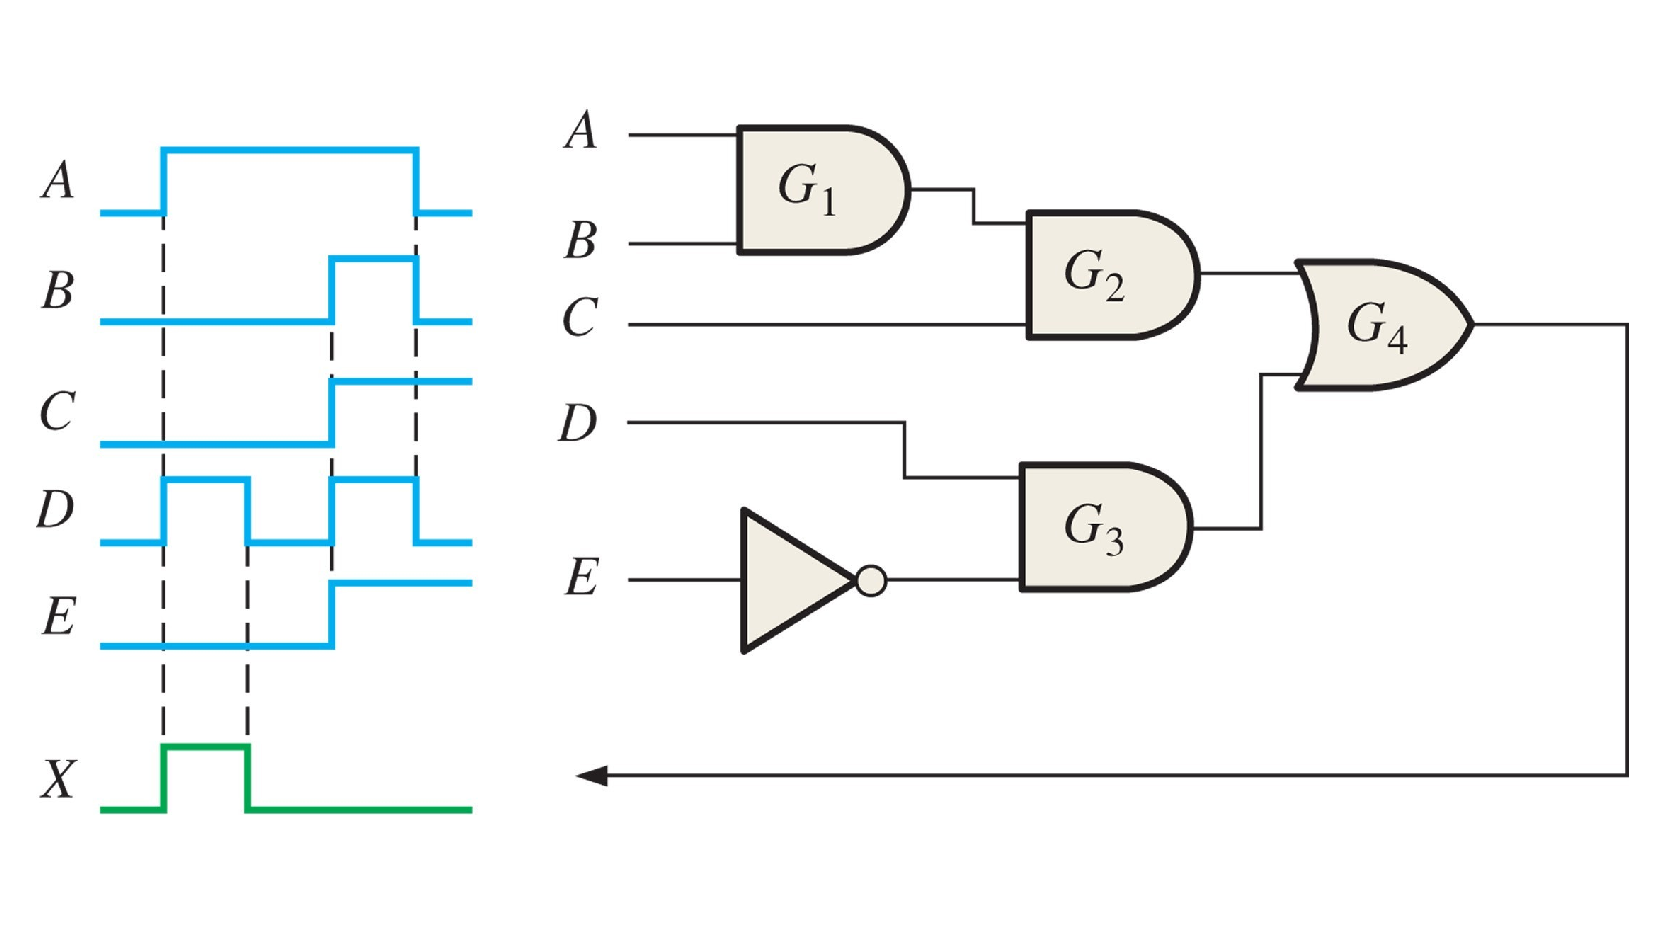
\includegraphics[width=0.4\textwidth]{figures/troubleshoot.pdf}
\caption{\label{fig:gates1} A domain-5 logic function needs debugging.}
\end{figure}

\section{Chapter 6 - Functions of Combinational Logic}
\label{sec:comb2}

\begin{figure}[ht]
\centering
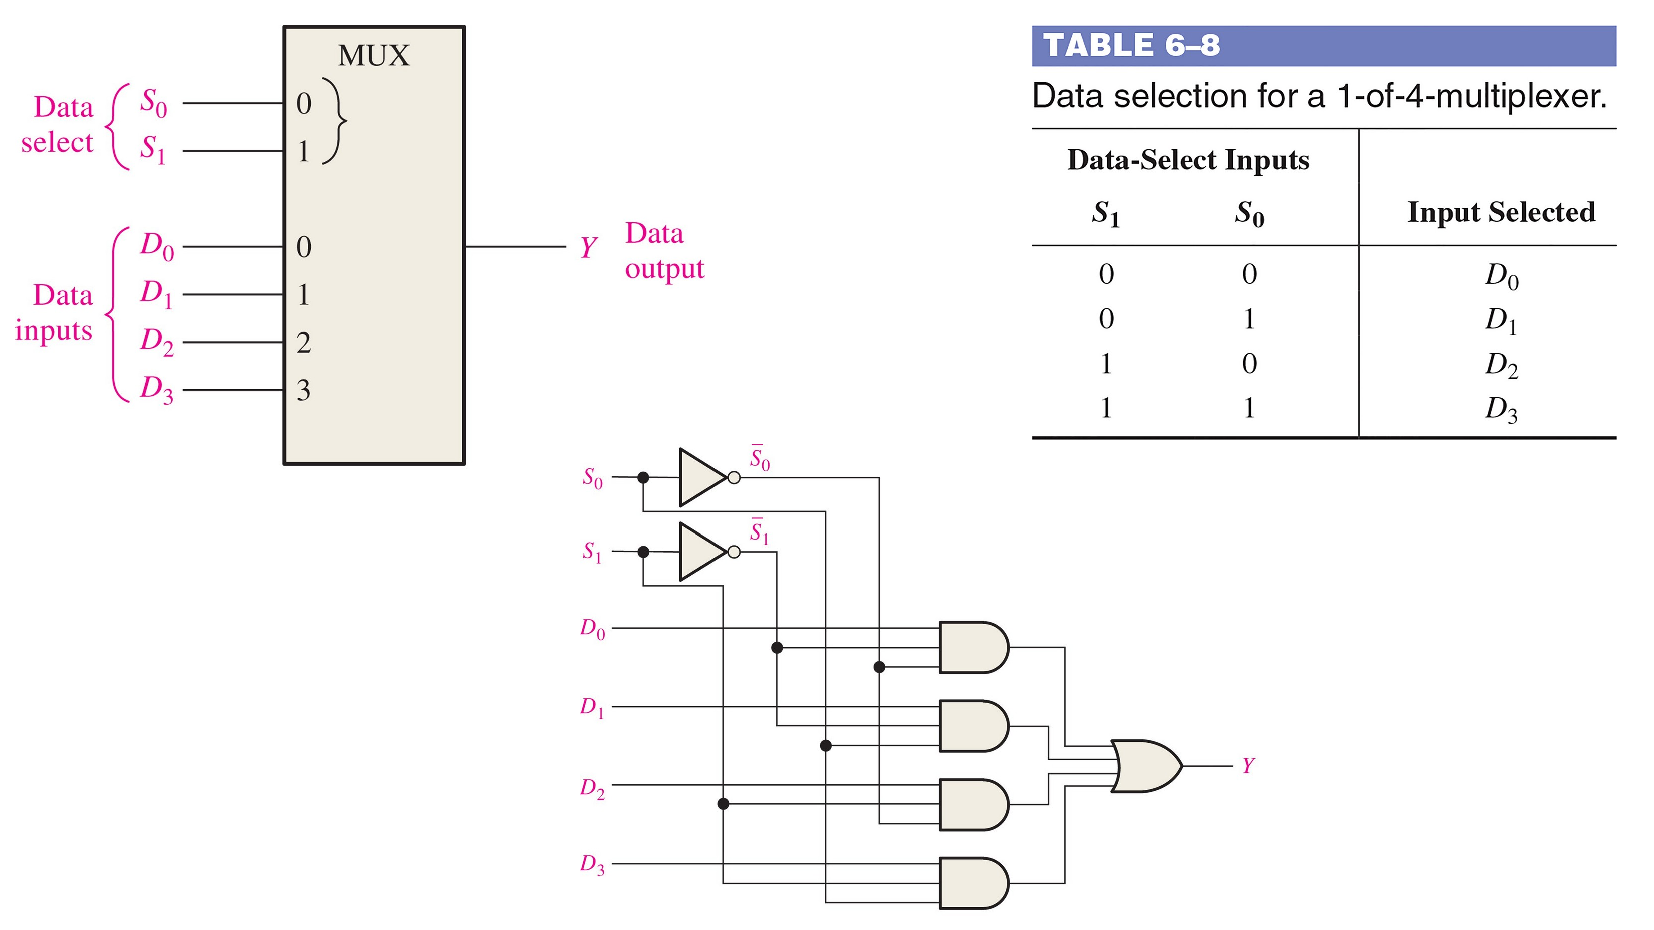
\includegraphics[width=0.5\textwidth]{figures/mux4.pdf}
\caption{\label{fig:mux4} A 1-of-4 multiplexer (mux) logic function: function block, truth table, and gate diagram.}
\end{figure}

\begin{enumerate}
\item Consider Fig. \ref{fig:mux4}, in which the 1-of-4 mux is reviewed.  Imagine a camera system (like Zoom only with firmware) in which you are switching between four data feeds from four cameras by holding down one of four different keys.  Design a circuit using an encoder and a 1-of-4 mux to switch between four bitstreams on active-LOW keypresses from four keys. Show the encoder logic at the gate level.  \\ \vspace{3cm}
\item Using XNOR gates, we could create a comparator that is true if two 2-bit binary numbers are equal.  Starting with the 2-bit comparator, add logic that is true if $A>B$.  Add one final output that is the opposite of $A>B$ (so $A<B$)\footnote{Since this is a 2-bit system, you can enumerate all possible states, if that helps.}. \\ \vspace{3cm}
\end{enumerate}

\section{Chapter 7 - Latches, Flip-flops, and Timers}
\label{sec:latch}

\begin{figure}[ht]
\centering
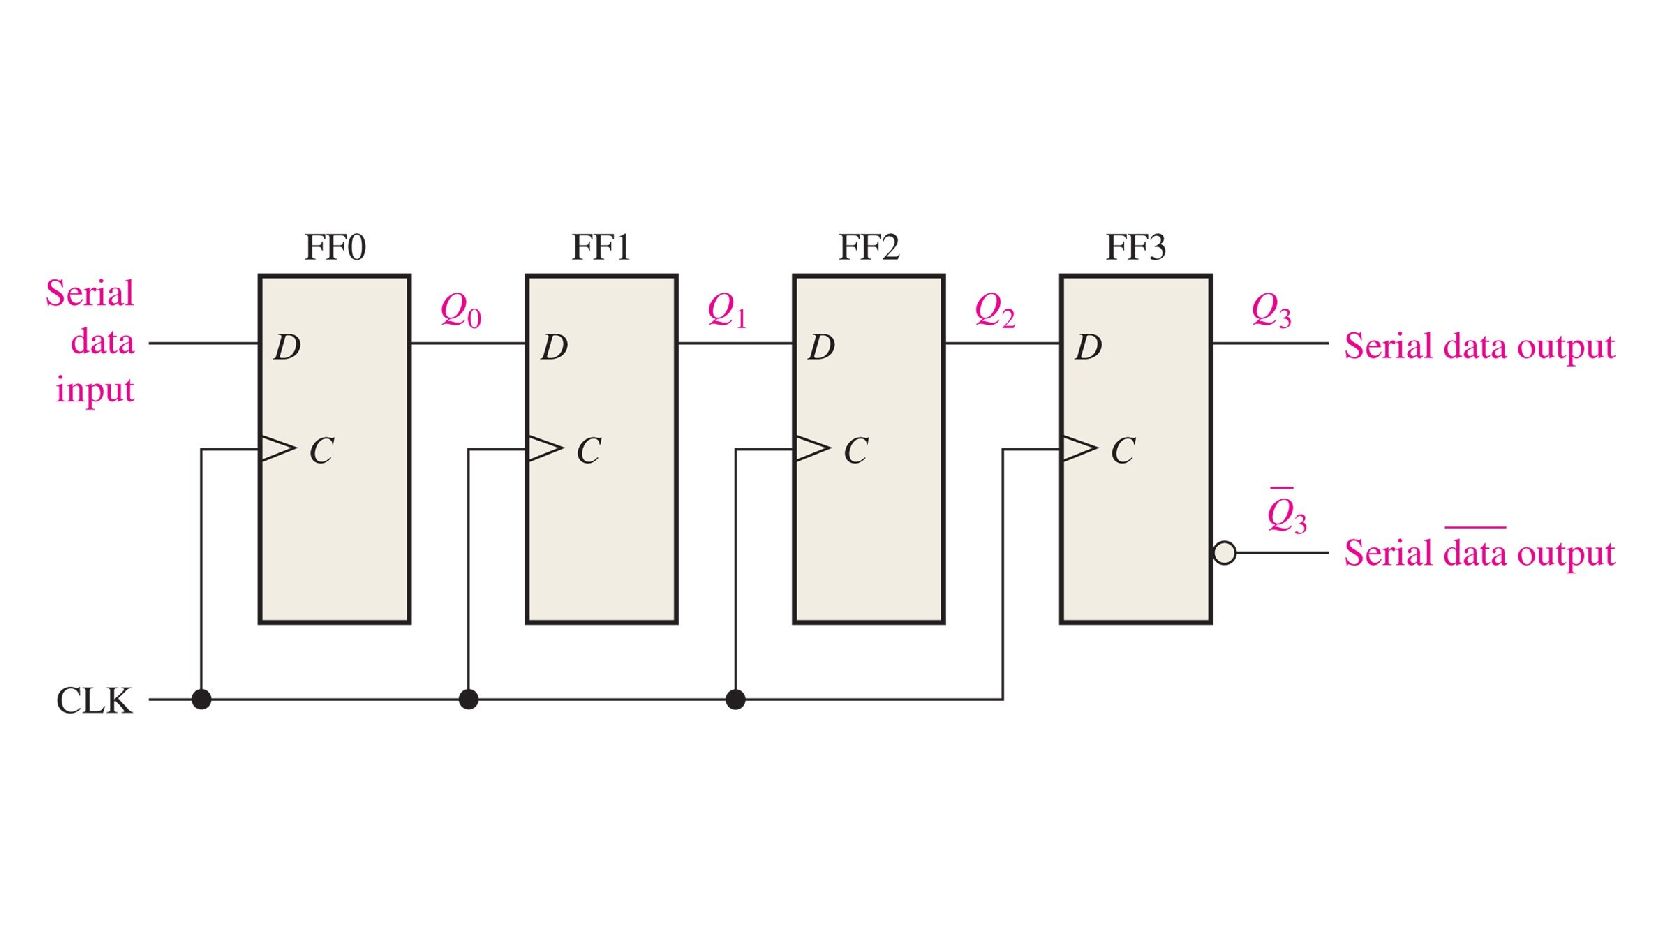
\includegraphics[width=0.5\textwidth,trim=0cm 2cm 0cm 2cm,clip=true]{figures/latches2.pdf}
\caption{\label{fig:latches} This is an example of a serial-in serial-out shift register.}
\end{figure}

\begin{enumerate}
\item Consider Fig. \ref{fig:latches}, in which four D flip-flops are connected in series to form a \textit{shift register.}  (a) Produce the timing diagram that occurs on the serial data output when all four D flip-flops are initially in the RESET state, and a single data bit arrives at the input with a constantly-running clock signal.  (b) Add an input that disables the clock to halt the shift register so that the data is stored.  Draw a timing diagram showing the shifting of 4 bits into the register and halting on the right clock cycle to store them. \\ \vspace{3cm}
\item Create a function block to represent the 4-bit shift register from the previous problem.  Now design a system that adds two binary numbers and stores the result in the shift register via a 1-of-4 multiplexer.  The mux is there to convert the \textit{parallel} data out of the adder to \textit{serial} data into the register. (Continue response on back).
\end{enumerate}

\end{document}